\chapter{Modelli a parametri concentrati}
\section{Segnali elettrici nel dominio del tempo e della frequenza}
Un segnale elettrico propagante lungo una struttura fisica varia sia nello spazio sia nel tempo. Nel caso ideale di un'\textbf{onda sinusoidale} che si propaga in un mezzo omogeneo privo di dispersione, il segnale manifesta una periodicità spaziale, con periodo pari alla lunghezza d'onda $\lambda$, e una periodicità temporale, con periodo $T$.

Le relazioni fondamentali che legano la frequenza $f$, il periodo $T$, la pulsazione $\omega$ e la lunghezza d'onda $\lambda$ sono definite da:
\[
\omega = 2\pi f
\]
\[
f = \frac{1}{T}
\]
\[
\lambda = \frac{v_p}{f}
\]
In un mezzo dielettrico assimilabile allo spazio libero o all'aria, la velocità di fase $v_p$ coincide con la velocità della luce nel vuoto $c \approx 3 \cdot 10^8\text{ m/s}$. La velocità della luce non è mai stata misurata sperimentalmente su una singola tratta di sola andata, ma su percorsi chiusi di andata e ritorno con riflessione su specchio; l'assunto di simmetria e isotropia della velocità lungo l'andata e il ritorno costituisce un'ipotesi fondamentale della relatività ristretta formulata da Albert Einstein, pienamente operativa e verificata nell'ingegneria applicata.

La lunghezza d'onda varia in proporzione inversa rispetto alla frequenza:
\begin{itemize}
    \item \textbf{$50\text{ Hz}$} $\rightarrow$ $\lambda = 6000\text{ km}$, frequenza di rete elettrica e alimentatori.
    \item \textbf{$30\text{ kHz}$} $\rightarrow$ $\lambda = 10\text{ km}$, onde lunghe e disturbi condotti a bassa frequenza.
    \item \textbf{$300\text{ kHz}$} $\rightarrow$ $\lambda = 1\text{ km}$, linee di trasmissione regionali.
    \item \textbf{$30\text{ MHz}$} $\rightarrow$ $\lambda = 10\text{ m}$, transizione tra disturbi condotti e disturbi irradiati.
    \item \textbf{$300\text{ MHz}$} $\rightarrow$ $\lambda = 1\text{ m}$, insorgenza del campo irradiato significativo e soglia normativa.
    \item \textbf{$3\text{ GHz}$} $\rightarrow$ $\lambda = 10\text{ cm}$, dimensioni comparabili a schede a circuito stampato e dispositivi portatili.
    \item \textbf{$30\text{ GHz}$} $\rightarrow$ $\lambda = 1\text{ cm}$, microstrisce, package di circuiti integrati e frequenze millimetriche.
\end{itemize}
Nell'intervallo compreso tra $30\text{ MHz}$ e $30\text{ GHz}$, $\lambda$ assume valori direttamente comparabili con le dimensioni geometriche delle interconnessioni e degli oggetti di impiego comune, in particolare linee elettriche ed elettroniche. La natura dei fenomeni dipende dal rapporto dimensionale tra la grandezza fisica dell'oggetto e la lunghezza d'onda.
\begin{figure}[H]
	\centering
	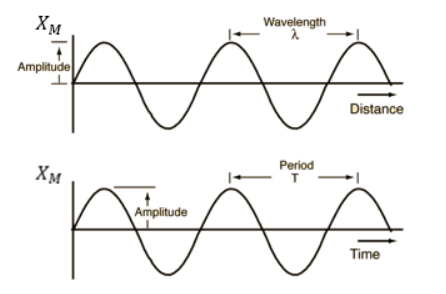
\includegraphics[width=0.5\linewidth]{immagini/parametri_concentrati1}
\end{figure}
Un segnale periodico $x(t)$ non sinusoidale di periodo $T$ e frequenza fondamentale $f_0 = \frac{1}{T}$ può essere espresso in \textbf{serie di Fourier} come somma discreta della componente continua e delle armoniche sinusoidali a frequenze multiple intere di $f_0$:
\[
x(t) = X_0 \sin(\varphi_0) + \sum_{n=1}^{\infty} X_n \sin(2\pi n f_0 t + \varphi_n) = \sum_{n=0}^{\infty} X_n \sin(2\pi n f_0 t + \varphi_n)
\]
Lo spettro di un segnale periodico è discreto:
\begin{itemize}
    \item \textbf{Spettro di ampiezza} $\rightarrow$ sequenza a righe dei coefficienti $X_n$ valutati alle frequenze discrete $n f_0$.
    \item \textbf{Spettro di fase} $\rightarrow$ sequenza a righe delle fasi iniziali $\varphi_n$ associate a ciascuna riga spettrale alle frequenze $n f_0$.
\end{itemize}
\begin{figure}[H]
	\centering
	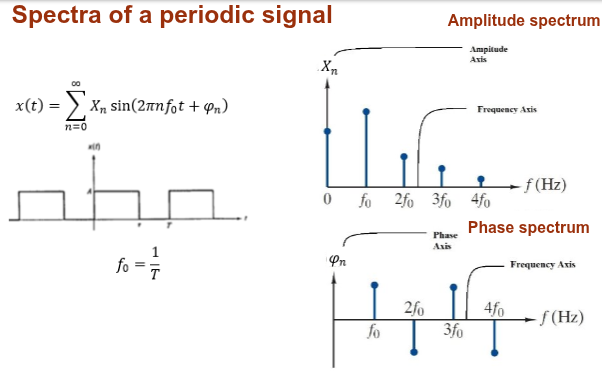
\includegraphics[width=0.8\linewidth]{immagini/parametri_concentrati2}
\end{figure}

Nei circuiti digitali reali, le commutazioni logiche, quali i treni di impulsi di clock per il trasferimento dati, presentano una forma d'onda trapezoidale con fronti di salita e di discesa non ripidi:
\begin{itemize}
    \item \textbf{$T_r$} $\rightarrow$ tempo di salita del segnale.
    \item \textbf{$T_f$} $\rightarrow$ tempo di discesa del segnale.
    \item \textbf{$T$} $\rightarrow$ periodo di ripetizione del segnale.
\end{itemize}
\begin{figure}[H]
	\centering
	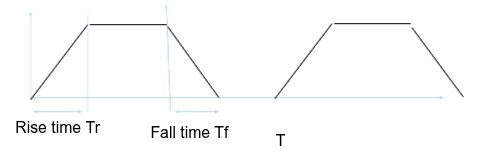
\includegraphics[width=0.6\linewidth]{immagini/parametri_concentrati3}
\end{figure}
I parametri $1/T_r$ e $1/T_f$ individuano dove si colloca il contenuto spettrale significativo in alta frequenza: minore è il tempo di salita, più estese sono le armoniche ad alta frequenza prodotte dal segnale. Nell'analisi di un segnale di clock con frequenza fondamentale a $1\text{ GHz}$, l'osservazione della sola fondamentale è insufficiente; per evitare la distorsione del segnale campionato, occorre acquisire almeno fino alla settima o nona armonica, corrispondente a $7\text{ GHz} - 9\text{ GHz}$, richiedendo oscilloscopi di misura commerciali dotati di una banda passante di almeno $10\text{ GHz}$.

Nel caso di un segnale aperiodico generico, lo sviluppo a righe discrete si generalizza nell'integrale della \textbf{trasformata di Fourier}: lo spettro di un segnale non periodico è continuo lungo l'asse delle frequenze.
\begin{figure}[H]
	\centering
	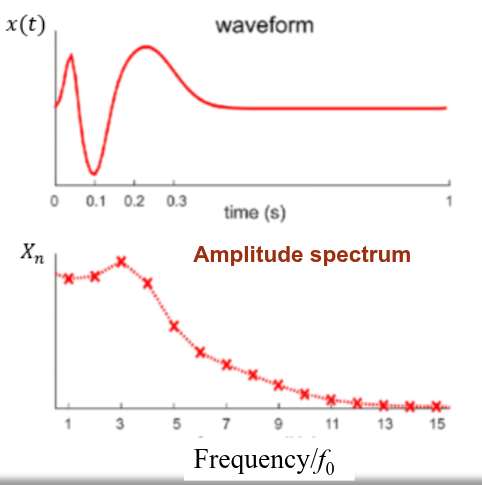
\includegraphics[width=0.4\linewidth]{immagini/parametri_concentrati4}
\end{figure}

La \textbf{banda di un segnale} individua l'intervallo di frequenze che racchiude le componenti spettrali dominanti. La definizione a $3\text{ dB}$ identifica l'intervallo:
\[
B = f_H - f_L
\]
in cui l'ampiezza dello spettro si mantiene superiore a $X_{\max}/\sqrt{2} \approx 0.707\, X_{\max}$, corrispondente a un'attenuazione di $-3\text{ dB}$.
\begin{figure}[H]
	\centering
	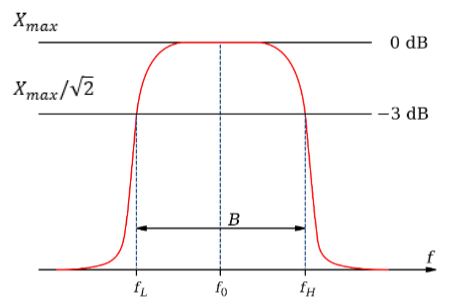
\includegraphics[width=0.5\linewidth]{immagini/parametri_concentrati5}
\end{figure}
Per gestire ampiezze caratterizzate da estesi ordini di grandezza, dal microvolt alle centinaia di volt, e frequenze nell'intervallo delle microonde, si impiega la \textbf{scala logaritmica in decibel}:
\[
V_{\text{dB,REF}} = 20 \log_{10}\left(\frac{V_X}{V_{\text{REF}}}\right)
\]
\[
I_{\text{dB,REF}} = 20 \log_{10}\left(\frac{I_X}{I_{\text{REF}}}\right)
\]
\[
P_{\text{dB,REF}} = 10 \log_{10}\left(\frac{P_X}{P_{\text{REF}}}\right)
\]
\begin{itemize}
    \item \textbf{$V_{\text{REF}}$} $\rightarrow$ tensione di riferimento, espressa in volt.
    \item \textbf{$V_X$} $\rightarrow$ tensione in scala lineare, espressa in volt.
    \item \textbf{$I_{\text{REF}}$} $\rightarrow$ corrente di riferimento, espressa in ampere.
    \item \textbf{$I_X$} $\rightarrow$ corrente in scala lineare, espressa in ampere.
    \item \textbf{$P_{\text{REF}}$} $\rightarrow$ potenza di riferimento, espressa in watt.
    \item \textbf{$P_X$} $\rightarrow$ potenza in scala lineare, espressa in watt.
\end{itemize}
Il coefficiente per la potenza è $10$ anziché $20$ poiché la potenza elettrica dipende dal quadrato della tensione o della corrente ($P \propto V^2$ oppure $P \propto I^2$); per le proprietà dei logaritmi, l'esponente quadratico diviene un fattore $2$ moltiplicativo che, applicato a $10$, garantisce la coerenza della scala.

Nei diagrammi di Bode, le pendenze asintotiche caratteristiche assumono i valori seguenti:
\begin{itemize}
    \item \textbf{$0\text{ dB/decade}$} $\rightarrow$ andamento costante indipendente dalla frequenza.
    \item \textbf{$+20\text{ dB/decade}$} $\rightarrow$ andamento proporzionale alla frequenza $f$, tipico del comportamento differenziatore o induttivo.
    \item \textbf{$-20\text{ dB/decade}$} $\rightarrow$ andamento proporzionale a $1/f$, corrispondente a un decadimento lineare con la frequenza, tipico del comportamento integratore o capacitivo.
    \item \textbf{$+40\text{ dB/decade}$} $\rightarrow$ andamento proporzionale al quadrato della frequenza $f^2$.
    \item \textbf{$-40\text{ dB/decade}$} $\rightarrow$ andamento proporzionale a $1/f^2$, corrispondente a un decadimento con il quadrato della frequenza.
    \item \textbf{$+10\text{ dB/decade}$} $\rightarrow$ andamento proporzionale alla radice quadrata della frequenza $\sqrt{f}$.
    \item \textbf{$-10\text{ dB/decade}$} $\rightarrow$ andamento proporzionale a $1/\sqrt{f}$, tipico dell'attenuazione introdotta dall'effetto pelle nei conduttori ad alta frequenza.
\end{itemize}
\begin{figure}[H]
	\centering
	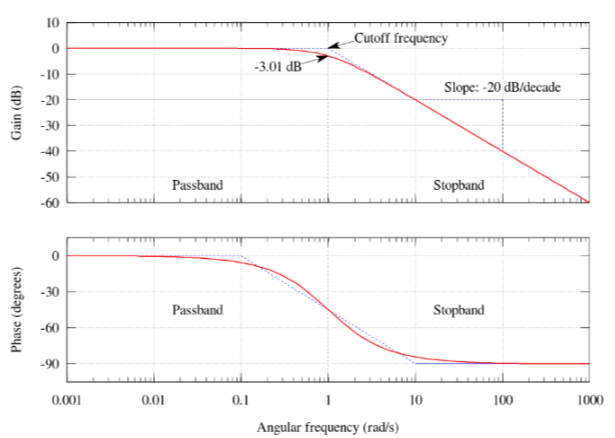
\includegraphics[width=0.6\linewidth]{immagini/parametri_concentrati6}
\end{figure}


\section{Filtraggio e risposta in frequenza dei sistemi lineari}
Un filtro, rappresentabile come sistema lineare tempo-invariante, è caratterizzato dalla funzione di trasferimento $H(f)$ o dalla risposta all'impulso $h(t)$. La relazione ingresso-uscita nel dominio della frequenza è un prodotto algebrico:
\[
Y(f) = H(f) \cdot X(f)
\]
A tale relazione corrisponde nel dominio temporale l'integrale di convoluzione:
\[
y(t) = h(t) * x(t)
\]
Operare nel dominio della frequenza semplifica l'analisi evitando la convoluzione temporale.
\begin{figure}[H]
	\centering
	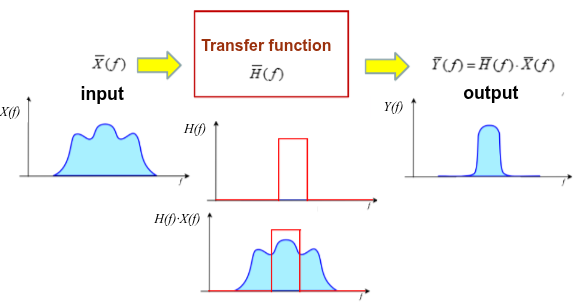
\includegraphics[width=0.6\linewidth]{immagini/parametri_concentrati7}
\end{figure}

I filtri si suddividono in due classi:
\begin{itemize}
    \item \textbf{Filtro ideale} $\rightarrow$ presenta guadagno unitario costante nella banda passante, attenuazione infinita nelle bande interdette e transizioni a gradino a pendenza infinita. Tale filtro non è realizzabile con componenti analogici discreti per vincoli di causalità; è realizzabile numericamente tramite elaborazione digitale su segnali campionati.
    \item \textbf{Filtro reale} $\rightarrow$ realizzato con componenti circuitali fisici, presenta un'attenuazione progressiva e continua attorno alla frequenza di taglio a $3\text{ dB}$.
\end{itemize}

Le configurazioni fondamentali dei filtri comprendono:
\begin{itemize}
    \item \textbf{Filtro passa-basso} $\rightarrow$ trasmette le frequenze inferiori alla frequenza di taglio attenuando le frequenze superiori.
    \item \textbf{Filtro passa-alto} $\rightarrow$ trasmette le frequenze superiori alla frequenza di taglio attenuando le frequenze inferiori.
    \item \textbf{Filtro passa-banda} $\rightarrow$ trasmette le frequenze comprese tra due frequenze di taglio attenuando quelle esterne.
    \item \textbf{Filtro arresta-banda} $\rightarrow$ attenua le frequenze comprese nella banda d'arresto trasmettendo quelle inferiori e superiori.
\end{itemize}
\begin{figure}[H]
	\centering
	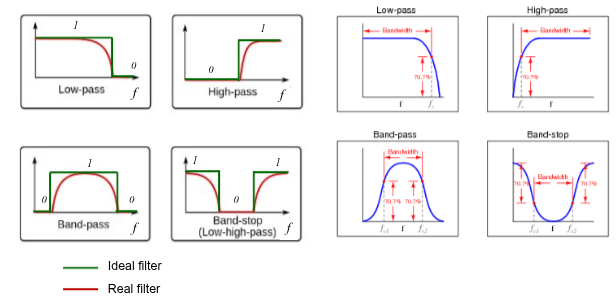
\includegraphics[width=0.6\linewidth]{immagini/parametri_concentrati8}
\end{figure}

L'applicazione di un filtro passa-basso elimina i disturbi ad alta frequenza, determinando un'apparente riduzione del disordine del segnale. Tale riduzione non viola il secondo principio della termodinamica poiché la diminuzione locale di entropia è permessa dall'informazione a priori iniettata nel sistema dal progettista in merito alla banda utile del segnale.
\begin{figure}[H]
	\centering
	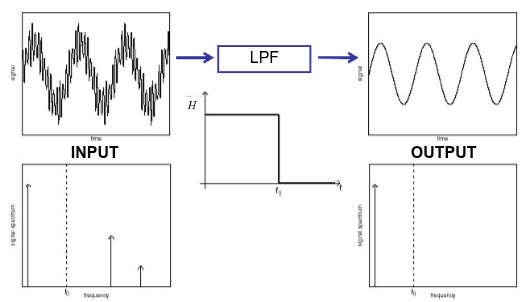
\includegraphics[width=0.6\linewidth]{immagini/parametri_concentrati9}
\end{figure}

La \textbf{legge di Ohm in regime sinusoidale} è espressa in termini fasoriali da:
\[
\bar{V} = \dot{Z} \bar{I}
\]
I parametri ideali dei componenti elementari presentano le impedenze seguenti:
\begin{itemize}
    \item \textbf{Resistore} $\rightarrow$ resistenza nominale $R$ [$\Omega$], con impedenza puramente reale $\dot{Z} = R$.
    \item \textbf{Condensatore} $\rightarrow$ capacità nominale $C$ [$\text{F}$], con impedenza $\dot{Z} = \frac{1}{j\omega C}$ e modulo:
    \[
    |\dot{Z}(\omega)| = \frac{1}{\omega C} = \frac{1}{2\pi f C}
    \]
    Per $\omega \to 0$ l'impedenza tende a infinito, realizzando un comportamento a circuito aperto; per $\omega \to \infty$ l'impedenza tende a zero, realizzando un comportamento a cortocircuito.
    \item \textbf{Induttore} $\rightarrow$ induttanza nominale $L$ [$\text{H}$], con impedenza $\dot{Z} = j\omega L$ e modulo:
    \[
    |\dot{Z}(\omega)| = \omega L = 2\pi f L
    \]
    Per $\omega \to 0$ l'impedenza tende a zero, realizzando un comportamento a cortocircuito; per $\omega \to \infty$ l'impedenza tende a infinito, realizzando un comportamento a circuito aperto.
\end{itemize}
\begin{figure}[H]
	\centering
	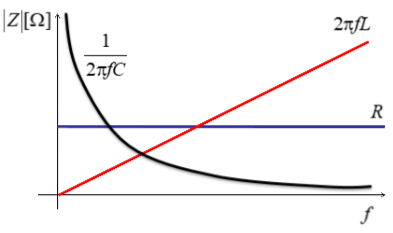
\includegraphics[width=0.5\linewidth]{immagini/parametri_concentrati10}
\end{figure}

\newpage
Nelle connessioni di impedenze:
\begin{itemize}
    \item \textbf{Connessione serie} $\rightarrow$ due impedenze $\dot{Z}_1$ e $\dot{Z}_2$ sono percorse dalla corrente $\bar{I}_{tot}$, con tensione complessiva $\bar{V}_{tot} = \bar{V}_1 + \bar{V}_2$. Se $|\dot{Z}_1| \ll |\dot{Z}_2|$, l'impedenza $\dot{Z}_1$ è trascurabile e si ha $\bar{V}_2 \approx \bar{V}_{tot}$.
    \item \textbf{Connessione parallelo} $\rightarrow$ due impedenze $\dot{Z}_1$ e $\dot{Z}_2$ sono sottoposte alla tensione $\bar{V}_{tot}$, con corrente complessiva $\bar{I}_{tot} = \bar{I}_1 + \bar{I}_2$. Se $|\dot{Z}_1| \gg |\dot{Z}_2|$, l'impedenza $\dot{Z}_1$ è trascurabile e si ha $\bar{I}_2 \approx \bar{I}_{tot}$.
\end{itemize}
\begin{figure}[H]
	\centering
	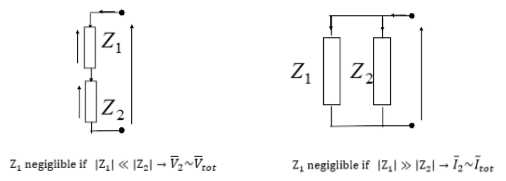
\includegraphics[width=0.6\linewidth]{immagini/parametri_concentrati11}
\end{figure}

Vediamo di seguito, un \textbf{esempio di filtro passa-basso} realizzato con un RC serie, in cui la tensione di ingresso $\bar{V}_i(\omega)$ alimenta il ramo serie di $R$ e $C$, con tensione di uscita $\bar{V}_o(\omega)$ prelevata ai capi di $C$:
\[
\bar{H}(\omega) = \frac{\bar{V}_o(\omega)}{\bar{V}_i(\omega)} = \frac{\frac{1}{j\omega C}}{R + \frac{1}{j\omega C}} = \frac{1}{1 + j\omega RC}
\]
Il modulo della funzione di trasferimento è:
\[
H(\omega) = |\bar{H}(\omega)| = \frac{1}{\sqrt{1 + (\omega RC)^2}}
\]
Alla pulsazione di taglio a $-3\text{ dB}$:
\[
\omega_{3\text{dB}} = \frac{1}{RC}
\]
il modulo vale:
\[
H(\omega_{3\text{dB}}) = \frac{1}{\sqrt{2}} \approx 0.707 \implies H_{\text{dB}} = -3\text{ dB}
\]
La banda passante a $3\text{ dB}$ coincide con $\omega_{3\text{dB}} = \frac{1}{RC}$.
\begin{figure}[H]
	\centering
	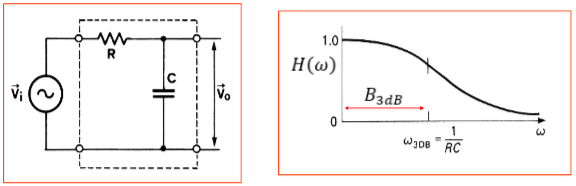
\includegraphics[width=0.6\linewidth]{immagini/parametri_concentrati12}
\end{figure}

Nel \textbf{filtro passa-banda RLC serie}, una maglia chiusa racchiude un generatore $\bar{V}_{in}(\omega)$, un condensatore $C$, un induttore $L$ e un resistore $R$, con tensione d'uscita $\bar{V}_{out}(\omega)$ prelevata ai capi del resistore $R$:
\[
\bar{H}(\omega) = \frac{\bar{V}_{out}(\omega)}{\bar{V}_{in}(\omega)} = \frac{R}{R + j\omega L + \frac{1}{j\omega C}} = \frac{1}{1 + j\left(\frac{\omega L}{R} - \frac{1}{\omega RC}\right)}
\]
Il modulo della risposta in frequenza è:
\[
H(\omega) = |\bar{H}(\omega)| = \frac{1}{\sqrt{1 + \left(\frac{\omega L}{R} - \frac{1}{\omega RC}\right)^2}}
\]
La condizione di risonanza si realizza all'annullarsi della reattanza totale della maglia:
\[
\frac{\omega L}{R} - \frac{1}{\omega RC} = 0 \iff \omega L = \frac{1}{\omega C}
\]
La pulsazione di risonanza è:
\[
\omega_r = \frac{1}{\sqrt{LC}}
\]
Alla risonanza, la funzione di trasferimento assume modulo unitario:
\[
H(\omega_r) = 1
\]
Il fattore di merito $Q_f$ del circuito è definito da:
\[
Q_f = \frac{\omega_r L}{R} = \frac{1}{\omega_r RC}
\]
La larghezza di banda passante a $3\text{ dB}$ è determinata da:
\[
B_{3\text{dB}} = \frac{\omega_r}{Q_f}
\]
All'aumentare del fattore di merito $Q_f$, corrispondente a valori decrescenti della resistenza dissipativa $R$, la curva di risposta spettrale mostra un picco più stretto ed una banda passante ridotta, determinando una maggiore selettività del filtro.
\begin{figure}[H]
	\centering
	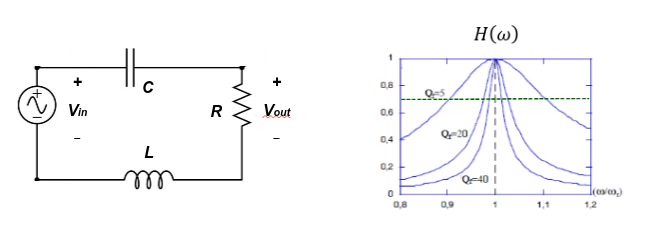
\includegraphics[width=0.7\linewidth]{immagini/parametri_concentrati13}
\end{figure}


\section{Criteri di scelta tra modelli a parametri concentrati e modelli a parametri distribuiti}
La formulazione elettromagnetica delle interconnessioni si articola in due modelli:
\begin{itemize}
    \item \textbf{Modello a parametri concentrati} $\rightarrow$ assume che la tensione e la corrente siano definite univocamente ai morsetti del componente e che il tempo di propagazione dell'onda elettromagnetica lungo le dimensioni fisiche della struttura sia trascurabile rispetto ai tempi caratteristici del segnale.
    \item \textbf{Modello a parametri distribuiti} $\rightarrow$ si adotta quando la propagazione non è istantanea, richiedendo la descrizione spaziale continua mediante le equazioni delle linee di trasmissione o le equazioni di Maxwell complete.
\end{itemize}
La scelta tra i due modelli dipende dal fatto che la dimensione fisica dell'oggetto sia o meno paragonabile alla lunghezza d'onda $\lambda$.

Si identificano quattro regimi elettromagnetici fondamentali:
\begin{itemize}
    \item \textbf{DC} $\rightarrow$ \textbf{regime stazionario} a frequenza nulla ($f = 0$), privo di variazioni temporali e di effetti propagativi; modellazione mediante sole resistenze pure dissipative.
    \item \textbf{EQS} $\rightarrow$ \textbf{regime elettro-quasi-statico} alle frequenze intermedie con propagazione trascurabile; dominano le cariche elettriche e l'accoppiamento reciproco è principalmente capacitivo, modellato con ammettenze in parallelo $Y(\omega)$ e resistenze.
    \item \textbf{MQS} $\rightarrow$ \textbf{regime magneto-quasi-statico} alle frequenze intermedie con propagazione trascurabile; dominano le correnti elettriche e l'accoppiamento reciproco è principalmente induttivo, modellato con impedenze in serie $Z(\omega)$ e resistenze.
    \item \textbf{FW} $\rightarrow$ \textbf{full wave} ad alte frequenze; lo scambio dinamico continuo tra campo elettrico e campo magnetico rende dominanti i ritardi di propagazione, imponendo modelli a parametri distribuiti.
\end{itemize}
\begin{figure}[H]
	\centering
	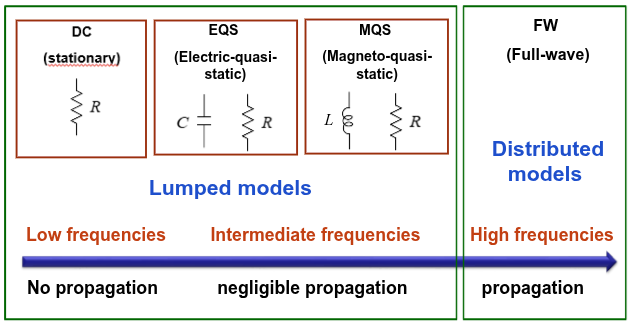
\includegraphics[width=0.7\linewidth]{immagini/parametri_concentrati14}
\end{figure}

Considerando una linea bifilare formata da due conduttori cilindrici paralleli di raggio $a$, interasse $d$ e lunghezza $l$:
\begin{figure}[H]
	\centering
	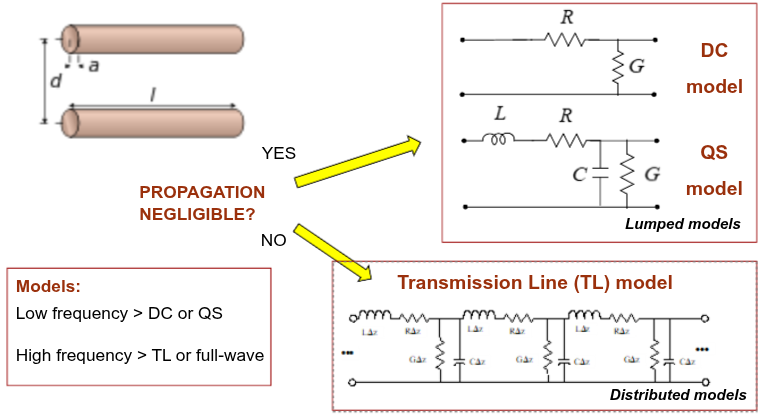
\includegraphics[width=0.7\linewidth]{immagini/parametri_concentrati15}
\end{figure}
\begin{itemize}
    \item Se la propagazione è trascurabile (basse frequenze, circuito elettricamente corto):
    \begin{itemize}
        \item Nel modello DC: una resistenza serie $R$ sul conduttore superiore e una conduttanza in parallelo $G$ dovuta alle perdite nel dielettrico interposto tra i due conduttori.
        \item Nel modello QS: un'induttanza serie $L$ e una resistenza serie $R$ lungo il conduttore, associate a una capacità trasversale $C$ e una conduttanza trasversale $G$ in parallelo tra i conduttori.
    \end{itemize}
    \item Se la propagazione non è trascurabile (alte frequenze, circuito elettricamente lungo):
    \begin{itemize}
        \item Modello a parametri distribuiti: modello della linea di trasmissione basato sulle equazioni dei telegrafisti con parametri distribuiti per unità di lunghezza o formulazioni full-wave.
    \end{itemize}
\end{itemize}

Il criterio quantitativo per la scelta tra modelli concentrati e distribuiti si basa sulla lunghezza elettrica ed è articolato nelle seguenti fasi:
\begin{enumerate}
    \item Determinazione della dimensione geometrica massima del sistema, indicata con $l_{\max}$.
    \item Identificazione della massima frequenza significativa del segnale, indicata con $f_{\max}$.
    \item Calcolo della minima lunghezza d'onda associata:
    \[
    \lambda_{\min} = \frac{v_p}{f_{\max}}
    \]
    essendo $v_p$ la velocità di fase nel mezzo di propagazione.
    \item Confronto tra la dimensione fisica $l_{\max}$ e la soglia critica:
    \[
    \frac{\lambda_{\min}}{10}
    \]
\end{enumerate}
\begin{figure}[H]
	\centering
	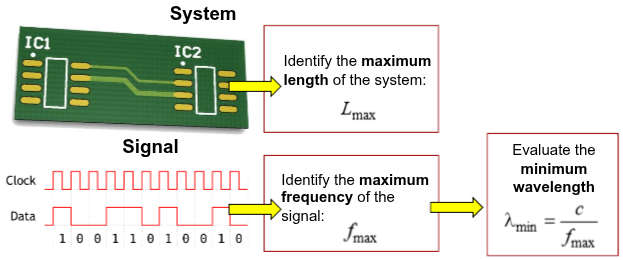
\includegraphics[width=0.6\linewidth]{immagini/parametri_concentrati16}
\end{figure}
Le condizioni discriminanti sono:
\begin{itemize}
    \item Se $l_{\max} < \frac{\lambda_{\min}}{10}$, il circuito è elettricamente corto $\rightarrow$ gli effetti propagativi sono trascurabili e i modelli a parametri concentrati sono applicabili.
    \item Se $l_{\max} \ge \frac{\lambda_{\min}}{10}$, il circuito è elettricamente lungo $\rightarrow$ gli effetti di propagazione sono significativi e richiedono modelli a parametri distribuiti.
\end{itemize}

La relatività della definizione di alta o bassa frequenza emerge dal confronto tra due casi applicativi di esempio riportati di seguito:
\begin{itemize}
    \item \textbf{Sovratensioni indotte da fulmine indiretto su linea aerea di potenza}:
    \begin{figure}[H]
    	\centering
    	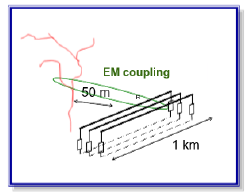
\includegraphics[width=0.3\linewidth]{immagini/parametri_concentrati20}
    \end{figure}
    \begin{itemize}
        \item Banda del segnale: $f \approx 1\text{ MHz}$.
        \item Velocità di propagazione: $v_p = c \approx 3 \cdot 10^8\text{ m/s}$.
        \item Lunghezza d'onda: $\lambda = \frac{c}{f} = \frac{3 \cdot 10^8\text{ m/s}}{10^6\text{ Hz}} = 300\text{ m}$.
        \item Lunghezza tipica del percorso esposto: $l = 1\text{ km} = 1000\text{ m}$.
        \item Rapporto dimensionale:
        \[
        l = 3.33\,\lambda \gg \frac{\lambda}{10}
        \]
        Il circuito è elettricamente lungo; alla frequenza di $1\text{ MHz}$ il sistema si trova in regime distribuito e impone la modellazione mediante equazioni dei telegrafisti per calcolare le sovratensioni indotte dalla scarica atmosferica caduta a breve distanza, ad esempio a $50\text{ m}$.
    \end{itemize}
    \item \textbf{Signal Integrity su microstriscia di circuito stampato}:
    \begin{figure}[H]
    	\centering
    	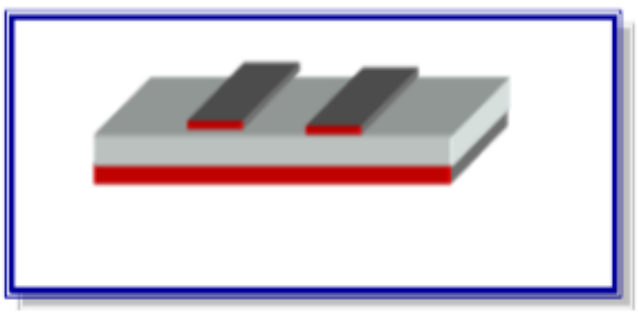
\includegraphics[width=0.23\linewidth]{immagini/parametri_concentrati21}
    \end{figure}
    
    \begin{itemize}
        \item Banda del segnale: $f \approx 20\text{ GHz}$.
        \item Velocità di propagazione su substrato dielettrico: $v_p \approx 1.7 \cdot 10^8\text{ m/s}$.
        \item Lunghezza d'onda: $\lambda = \frac{v_p}{f} \approx 10.5\text{ mm}$.
        \item Lunghezza di accoppiamento tra piste adiacenti: $l = 1\text{ mm}$.
        \item Rapporto dimensionale:
        \[
        l \approx 0.09\,\lambda < \frac{\lambda}{10}
        \]
        Il circuito è elettricamente corto; alla frequenza di $20\text{ GHz}$ la dimensione millimetrica consente di trattare l'accoppiamento tra piste vicine mediante parametri concentrati EQS o MQS. Se la pista attraversa l'intera scheda per una lunghezza di $20\text{ cm}$, essa diviene elettricamente lunga rispetto a $\lambda = 10.5\text{ mm}$, richiedendo il modello a linea di trasmissione.
    \end{itemize}
\end{itemize}

\section{Modellazione ad alta frequenza dei componenti reali}
Nelle condizioni nominali a bassa frequenza, nell'intervallo $0 - 10\text{ MHz}$, i componenti passivi operano secondo i modelli ideali dell'elettrotecnica. Nelle prove prescritte dalle norme di compatibilità elettromagnetica, quali le misure di emissione irradiata condotte tra $30\text{ MHz}$ e $1\text{ GHz}$, le strutture fisiche e i reofori introducono parametri parassiti che alterano la risposta in frequenza.

\subsection{Resistore reale ed effetti parassiti}
Un resistore commerciale presenta parametri parassiti legati alla geometria e ai reofori:
\begin{figure}[H]
	\centering
	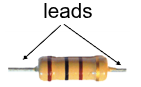
\includegraphics[width=0.2\linewidth]{immagini/parametri_concentrati23}
\end{figure}
\begin{itemize}
    \item \textbf{$R$} $\rightarrow$ resistenza nominale del componente.
    \item \textbf{$L_{\text{lead}}$} $\rightarrow$ induttanza parassita dei reofori metallici.
    \item \textbf{$C_{\text{lead}}$} $\rightarrow$ capacità parassita tra i reofori esterni.
    \item \textbf{$C_{\text{par}}$} $\rightarrow$ capacità parassita interna, indicata anche come $C_{\text{leakage}}$, associata all'avvolgimento del corpo resistivo o alle correnti di dispersione interne.
\end{itemize}

I modelli circuitali equivalenti si distinguono in:
\begin{itemize}
    \item \textbf{Modello di ordine 0} $\rightarrow$ circuito comprendente l'induttanza dei reofori $L_{\text{lead}}$ in serie al parallelo tra la resistenza nominale $R$ e la capacità parassita interna $C_{\text{par}}$.
    \begin{figure}[H]
    	\centering
    	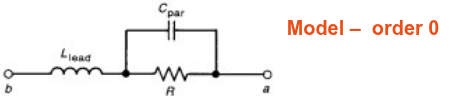
\includegraphics[width=0.5\linewidth]{immagini/parametri_concentrati18}
    \end{figure}
    
    \item \textbf{Modello di ordine 1} $\rightarrow$ modello più complesso che include esplicitamente la capacità parassita tra i morsetti esterni $C_{\text{lead}}$ in parallelo alla serie di $L_{\text{lead}}$ con la resistenza $R$ e la capacità interna distribuita $C_{\text{leakage}}$.
    \begin{figure}[H]
    	\centering
    	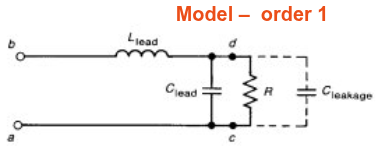
\includegraphics[width=0.4\linewidth]{immagini/parametri_concentrati19}
    \end{figure}
\end{itemize}


L'impedenza analitica $\hat{Z}(j\omega)$ del modello di ordine 0 è:
\[
\hat{Z}(j\omega) = j\omega L_{\text{lead}} + \frac{R}{1 + j\omega R C_{\text{par}}} = L_{\text{lead}} \frac{\frac{1}{L_{\text{lead}} C_{\text{par}}} - \omega^2 + j\frac{\omega}{R C_{\text{par}}}}{j\omega + \frac{1}{R C_{\text{par}}}}
\]
L'andamento del modulo dell'impedenza $|\hat{Z}(f)|$ in funzione della frequenza presenta tre regioni asintotiche:
\begin{figure}[H]
	\centering
	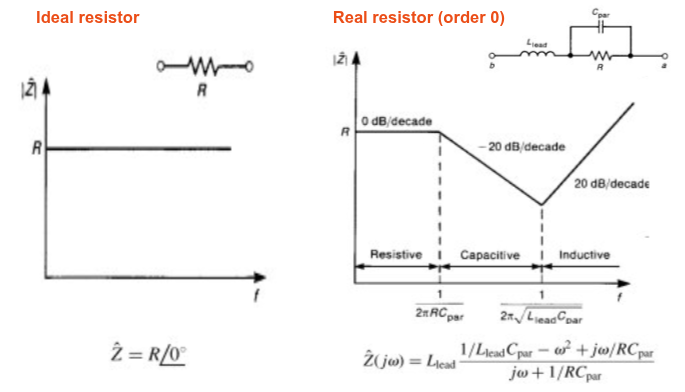
\includegraphics[width=0.7\linewidth]{immagini/parametri_concentrati22}
\end{figure}
\begin{enumerate}
    \item \textbf{Regione resistiva} $\rightarrow$ a basse frequenze ($f < f_1$), il modulo è costante e pari alla resistenza nominale:
    \[
    |\hat{Z}| = R
    \]
    con pendenza asintotica di $0\text{ dB/decade}$.
    \item \textbf{Regione capacitiva} $\rightarrow$ al di sopra della prima frequenza caratteristica:
    \[
    f_1 = \frac{1}{2\pi R C_{\text{par}}}
    \]
    la capacità parassita $C_{\text{par}}$ cortocircuita progressivamente la resistenza $R$; il modulo dell'impedenza decresce linearmente con la frequenza con pendenza di $-20\text{ dB/decade}$.
    \item \textbf{Regione induttiva} $\rightarrow$ oltre la frequenza di risonanza:
    \[
    f_r = \frac{1}{2\pi \sqrt{L_{\text{lead}} C_{\text{par}}}}
    \]
    l'induttanza parassita dei reofori $L_{\text{lead}}$ diviene dominante; il modulo cresce linearmente con la frequenza con una pendenza di $+20\text{ dB/decade}$.
\end{enumerate}


\subsection{Condensatore Reale e Frequenza di Risonanza Serie}
La struttura reale di un condensatore presenta parametri parassiti associati alle armature metalliche, al dielettrico e ai reofori:
\begin{figure}[H]
	\centering
	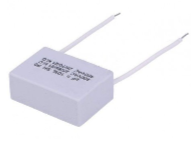
\includegraphics[width=0.2\linewidth]{immagini/parametri_concentrati24}
\end{figure}
\begin{itemize}
    \item \textbf{$C$} $\rightarrow$ capacità nominale del componente.
    \item \textbf{$L_{\text{lead}}$} $\rightarrow$ induttanza parassita dei reofori di collegamento.
    \item \textbf{$C_{\text{lead}}$} $\rightarrow$ capacità parassita presente tra i reofori esterni.
    \item \textbf{$R_{\text{plate}}$} $\rightarrow$ resistenza parassita delle armature metalliche.
    \item \textbf{$R_{\text{diel}}$} $\rightarrow$ resistenza di dispersione del dielettrico dovuta alle correnti di fuga.
    \item \textbf{$R_s$} $\rightarrow$ resistenza serie equivalente, che sintetizza in un unico elemento dissipativo le perdite ohmiche delle armature e del dielettrico.
\end{itemize}

I modelli circuitali equivalenti comprendono:
\begin{itemize}
    \item \textbf{Modello di ordine 0} $\rightarrow$ circuito RLC serie formato dalla capacità nominale $C$, dall'induttanza parassita dei reofori $L_{\text{lead}}$ e dalla resistenza serie equivalente $R_s$.
    \begin{figure}[H]
    	\centering
    	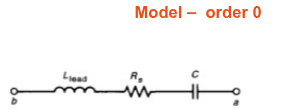
\includegraphics[width=0.4\linewidth]{immagini/parametri_concentrati25}
    \end{figure}
    
    \item \textbf{Modello di ordine 1} $\rightarrow$ circuito comprendente l'induttanza $L_{\text{lead}}$, la capacità tra i reofori $C_{\text{lead}}$, la resistenza delle armature $R_{\text{plate}}$ e la resistenza $R_{\text{diel}}$ posta in parallelo alla capacità nominale $C$.
    \begin{figure}[H]
    	\centering
    	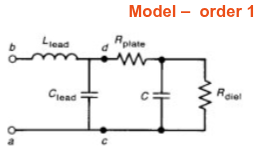
\includegraphics[width=0.3
    	\linewidth]{immagini/parametri_concentrati26}
    \end{figure}
\end{itemize}

L'espressione dell'impedenza per il modello di ordine 0 è:
\[
\hat{Z}_C(j\omega) = R_s + j\left(\omega L_{\text{lead}} - \frac{1}{\omega C}\right)
\]
L'andamento del modulo dell'impedenza $|\hat{Z}(f)|$ manifesta una caratteristica curva a V articolata in tre regioni sequenziali:
\begin{figure}[H]
	\centering
	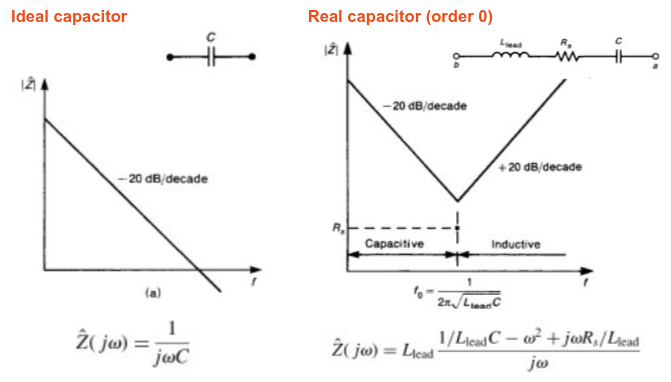
\includegraphics[width=0.7\linewidth]{immagini/parametri_concentrati27}
\end{figure}
\begin{enumerate}
    \item \textbf{Regione capacitiva} $\rightarrow$ a frequenze inferiori alla risonanza ($f < f_0$), prevale la capacità nominale $C$; il modulo dell'impedenza decresce all'aumentare della frequenza con pendenza pari a $-20\text{ dB/decade}$.
    \item \textbf{Frequenza di autorisonanza serie} $\rightarrow$ alla frequenza:
    \[
    f_0 = \frac{1}{2\pi \sqrt{L_{\text{lead}} C}}
    \]
    la reattanza induttiva compensa esattamente la reattanza capacitiva:
    \[
    \omega L_{\text{lead}} = \frac{1}{\omega C}
    \]
    La parte reattiva dell'impedenza si annulla e il modulo raggiunge il minimo assoluto, coincidendo con la sola resistenza serie equivalente:
    \[
    |\hat{Z}(f_0)| = R_s
    \]
    \item \textbf{Regione induttiva} $\rightarrow$ per frequenze superiori alla risonanza ($f > f_0$), l'induttanza dei reofori $L_{\text{lead}}$ prevale sulla capacità nominale; il modulo dell'impedenza cresce con pendenza asintotica di $+20\text{ dB/decade}$. Al di sopra di $f_0$, il componente cessa di operare come condensatore e assume a tutti gli effetti un comportamento induttivo.
\end{enumerate}

\subsection{Induttore Reale e Frequenza di Antirisonanza Parallelo}
Un induttore reale, realizzato tramite spire conduttrici in rame avvolte su un supporto, manifesta parametri parassiti dovuti alla resistività del filo e all'accoppiamento capacitivo tra spire contigue:
\begin{figure}[H]
	\centering
	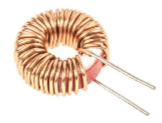
\includegraphics[width=0.2\linewidth]{immagini/parametri_concentrati28}
\end{figure}
\begin{itemize}
    \item \textbf{$L$} $\rightarrow$ induttanza nominale dell'avvolgimento.
    \item \textbf{$R_{\text{par}}$} $\rightarrow$ resistenza parassita ohmica del filo di rame delle spire.
    \item \textbf{$C_{\text{par}}$} $\rightarrow$ capacità parassita distribuita inter-spira presente tra le spire affiancate.
    \item \textbf{$L_{\text{lead}}$} $\rightarrow$ induttanza parassita dei terminali esterni.
    \item \textbf{$C_{\text{lead}}$} $\rightarrow$ capacità parassita tra i morsetti esterni.
\end{itemize}
A bassa frequenza e in corrente continua ($f = 0$), il modello classico dell'induttore fallisce: l'impedenza non è nulla, ma converge al valore finito della resistenza ohmica del filo di rame $R_{\text{par}}$.

I modelli circuitali equivalenti si articolano in:
\begin{itemize}
    \item \textbf{Modello di ordine 0} $\rightarrow$ ramo serie costituito dall'induttanza nominale $L$ e dalla resistenza parassita dell'avvolgimento $R_{\text{par}}$, collegato in parallelo con la capacità parassita inter-spira $C_{\text{par}}$.
    \begin{figure}[H]
    	\centering
    	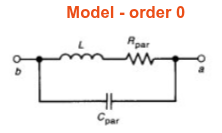
\includegraphics[width=0.3\linewidth]{immagini/parametri_concentrati29}
    \end{figure}
    
    \item \textbf{Modello di ordine 1} $\rightarrow$ circuito comprensivo dell'induttanza $L_{\text{lead}}$ e della capacità parassita $C_{\text{lead}}$ dei terminali esterni poste a monte della cella $L - R_{\text{par}} - C_{\text{par}}$.
    \begin{figure}[H]
    	\centering
    	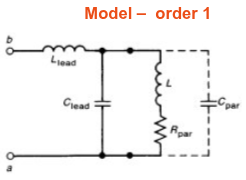
\includegraphics[width=0.3\linewidth]{immagini/parametri_concentrati30}
    \end{figure}
    
\end{itemize}

L'espressione analitica dell'impedenza per il modello di ordine 0 è:
\[
\hat{Z}_L(j\omega) = \frac{(R_{\text{par}} + j\omega L) \frac{1}{j\omega C_{\text{par}}}}{R_{\text{par}} + j\omega L + \frac{1}{j\omega C_{\text{par}}}} = R_{\text{par}} \frac{1 + j\frac{\omega L}{R_{\text{par}}}}{1 - \omega^2 L C_{\text{par}} + j\omega R_{\text{par}} C_{\text{par}}}
\]
L'andamento del modulo dell'impedenza $|\hat{Z}(f)|$ manifesta un profilo a campana:
\begin{figure}[H]
	\centering
	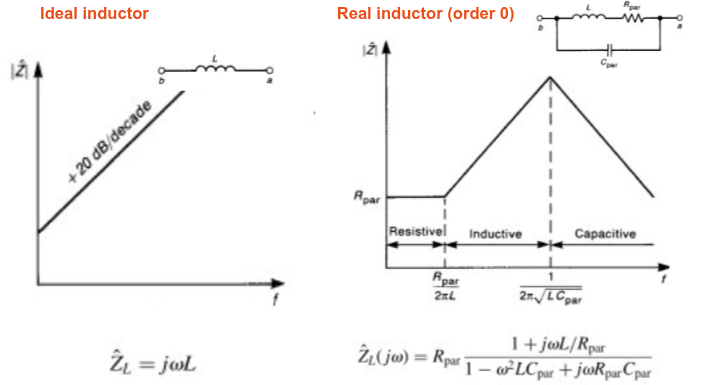
\includegraphics[width=0.7\linewidth]{immagini/parametri_concentrati31}
\end{figure}
\begin{enumerate}
    \item \textbf{Regione resistiva in continua} $\rightarrow$ per $f < f_1$, dove:
    \[
    f_1 = \frac{R_{\text{par}}}{2\pi L}
    \]
    l'impedenza è dominata dalla resistenza ohmica dell'avvolgimento ed è costante:
    \[
    |\hat{Z}| = R_{\text{par}}
    \]
    con pendenza asintotica di $0\text{ dB/decade}$.
    \item \textbf{Regione induttiva} $\rightarrow$ nell'intervallo $f_1 < f < f_r$, la reattanza dell'induttanza $L$ prevale su $R_{\text{par}}$; l'impedenza cresce linearmente con la frequenza con pendenza di $+20\text{ dB/decade}$.
    \item \textbf{Frequenza di antirisonanza parallelo} $\rightarrow$ alla frequenza:
    \[
    f_r = \frac{1}{2\pi \sqrt{L C_{\text{par}}}}
    \]
    il parallelo tra l'induttanza e la capacità inter-spira genera una risonanza parallelo in cui il modulo dell'impedenza raggiunge il suo valore massimo.
    \item \textbf{Regione capacitiva} $\rightarrow$ per frequenze superiori all'antirisonanza ($f > f_r$), la corrente fluisce prevalentemente attraverso la capacità distribuita inter-spira $C_{\text{par}}$; l'impedenza decresce all'aumentare della frequenza con pendenza di $-20\text{ dB/decade}$. L'induttore cessa di comportarsi da induttore e assume un comportamento capacitivo.
\end{enumerate}

\subsection{Indicazioni pratiche per i datasheet e la simulazione}
La scelta tra il modello equivalente di ordine 0 e quello di ordine 1 dipende dall'estensione dell'intervallo di frequenza operativo e dal livello di precisione richiesto dall'analisi di compatibilità elettromagnetica.

I costruttori di componenti elettronici forniscono nei datasheet i valori numerici dei parametri parassiti oppure le curve sperimentali dell'impedenza $|\hat{Z}(f)|$ misurate fino ad alcuni gigahertz mediante analizzatori di impedenza o analizzatori di reti vettoriali. Nelle simulazioni circuitali condotte con programmi quali SPICE, LTspice o MATLAB, l'inclusione dei parametri parassiti dei modelli di ordine superiore è indispensabile per diagnosticare risonanze indesiderate ed emissioni condotte o irradiate non previste nei modelli ideali.
